\section{Menus and a Splash Screen: The Front End}

\begin{itemize}
    \item Lots of screenshots!
    \item Explanation of menu system and splash screen, credits screen etc
    \item Discussion of some UI principles used
    \item mention sheen (GUI) framework from non-technical perspective (design / logic split etc).
\end{itemize}

\begin{figure*}[p]
	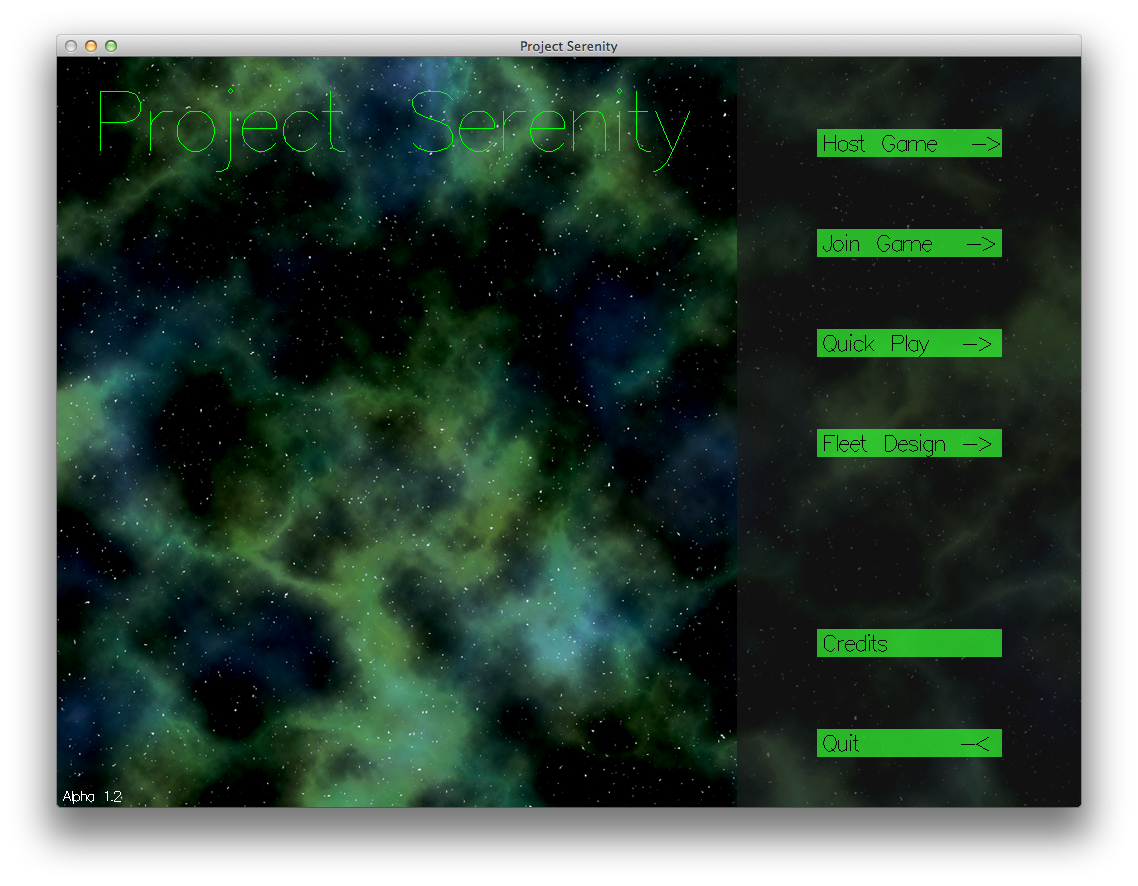
\includegraphics[width=15.5cm]{res/serenityscreens/01-mainmenu}
	\caption[Screenshot of the main menu]{Screenshot of the main menu.}
	\label{fig:mainmenu}
\end{figure*}

\begin{figure*}[p]
	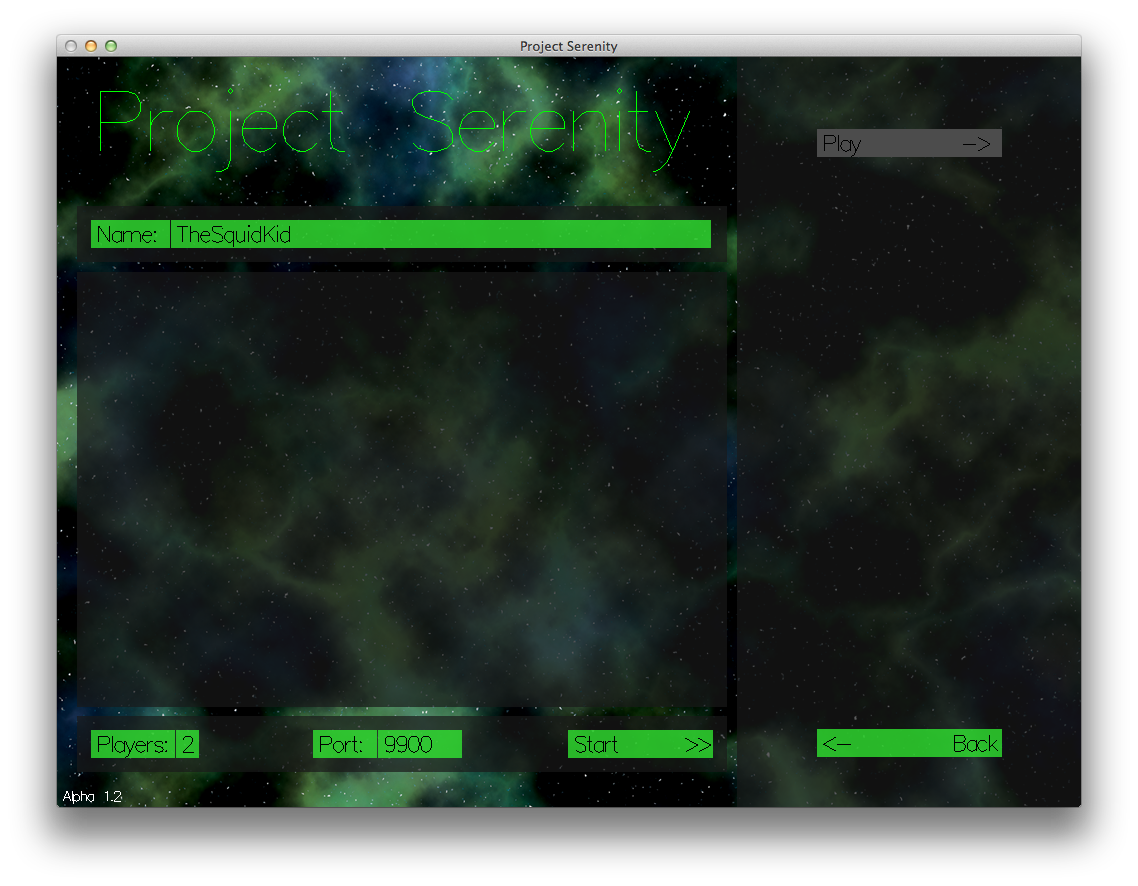
\includegraphics[width=15.5cm]{res/serenityscreens/02-host}
	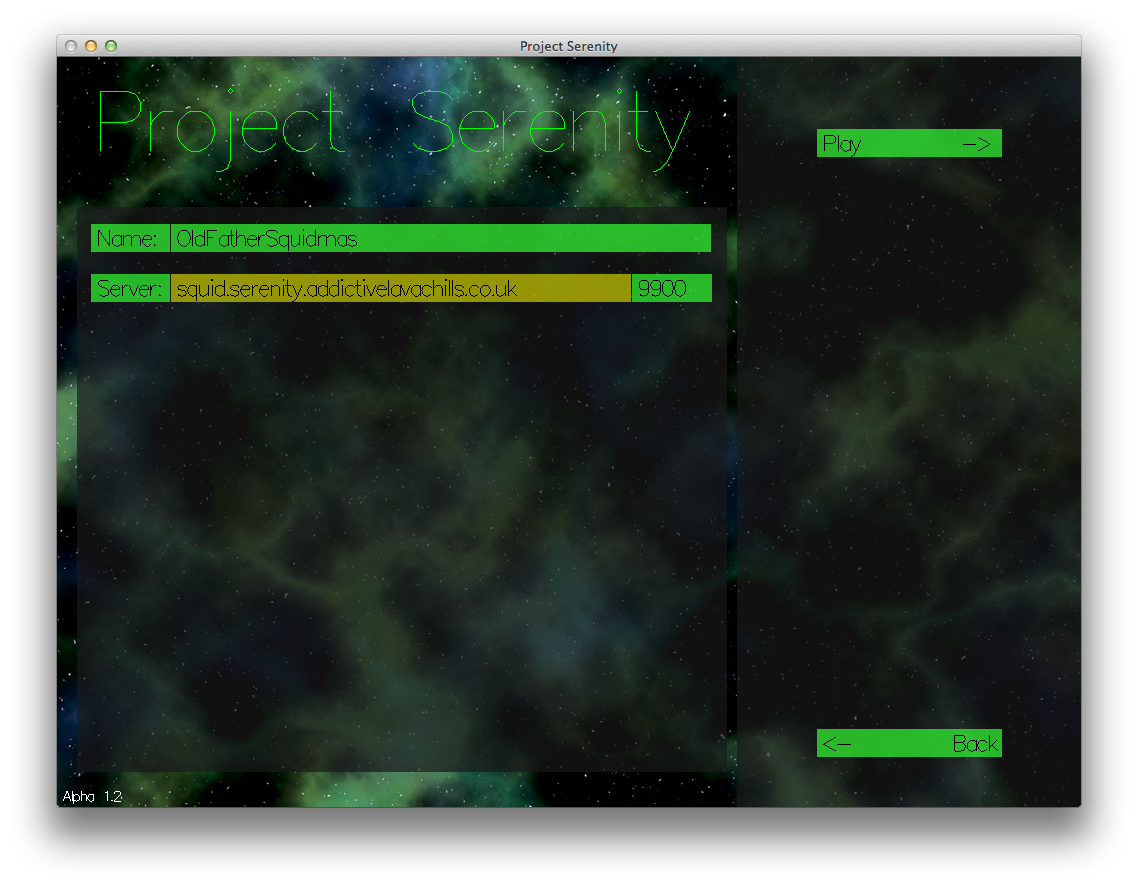
\includegraphics[width=15.5cm]{res/serenityscreens/03-join}
	\caption[Menus for hosting and joining battles]{Screenshot of the menus used to host and join battles.}
	\label{fig:hostjoin}
\end{figure*}

\begin{figure*}[p]
	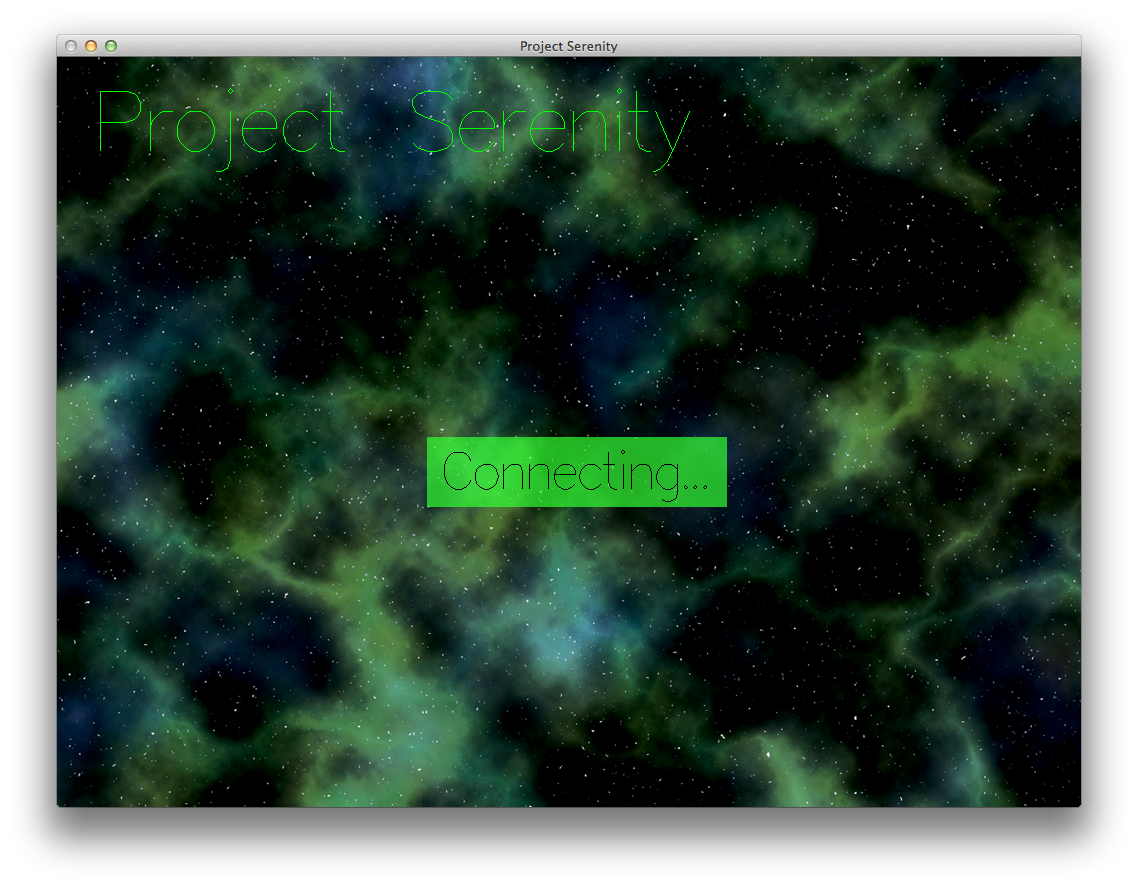
\includegraphics[width=15.5cm]{res/serenityscreens/06-connecting}
	\caption[Screenshot taken as a player connects to a server]{Screenshot taken as a player connects to a server.}
	\label{fig:connecting}
\end{figure*}

\begin{figure*}[p]
	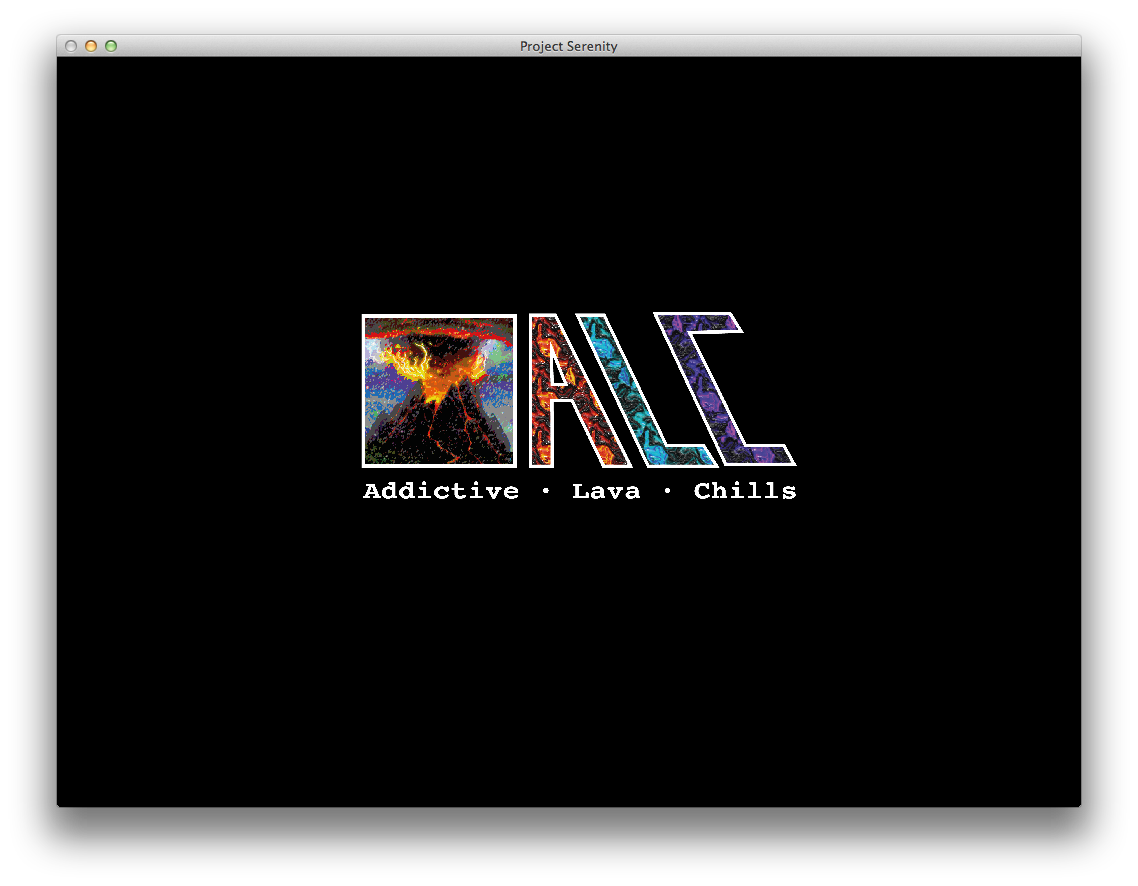
\includegraphics[width=15.5cm]{res/serenityscreens/07-splash1}
	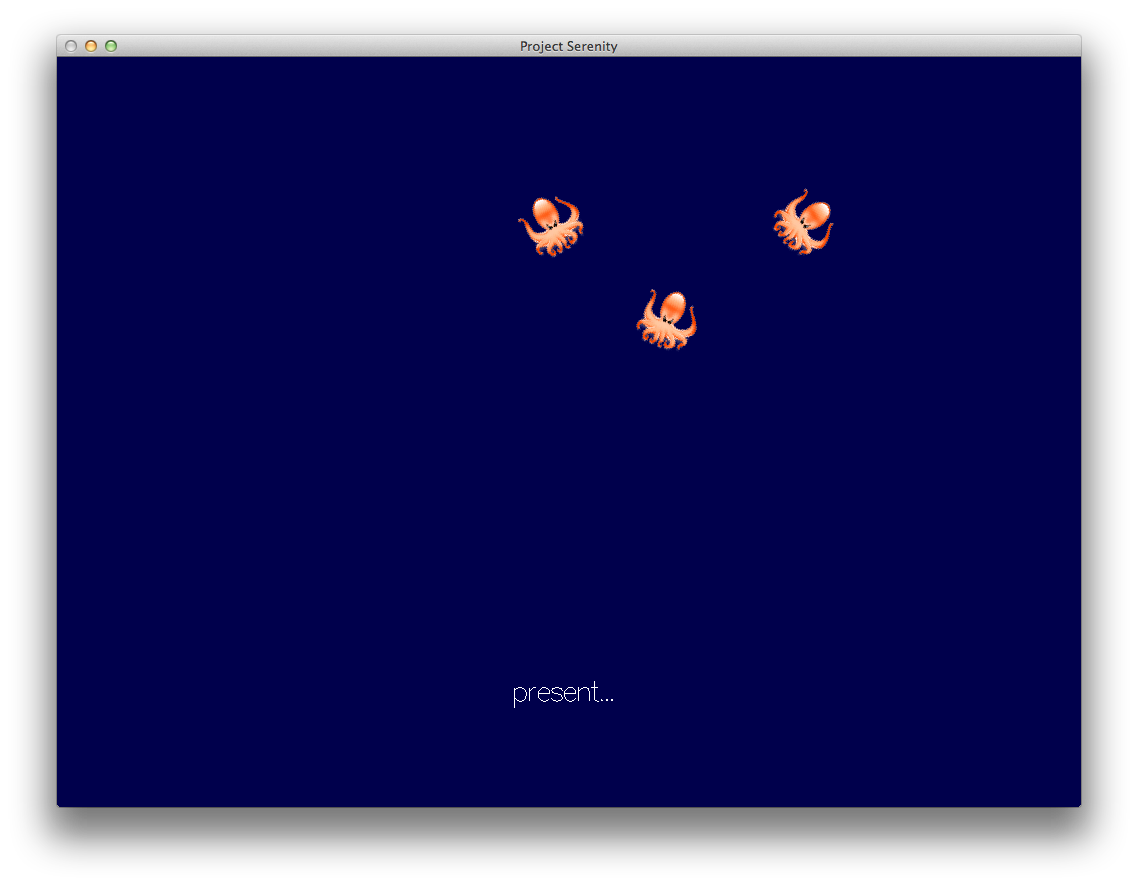
\includegraphics[width=15.5cm]{res/serenityscreens/08-splash2}
	\caption[Splash screens shown on launch]{Screenshot of the splash screens shown when the game is launched.}
	\label{fig:splash}
\end{figure*}

\begin{figure*}[p]
	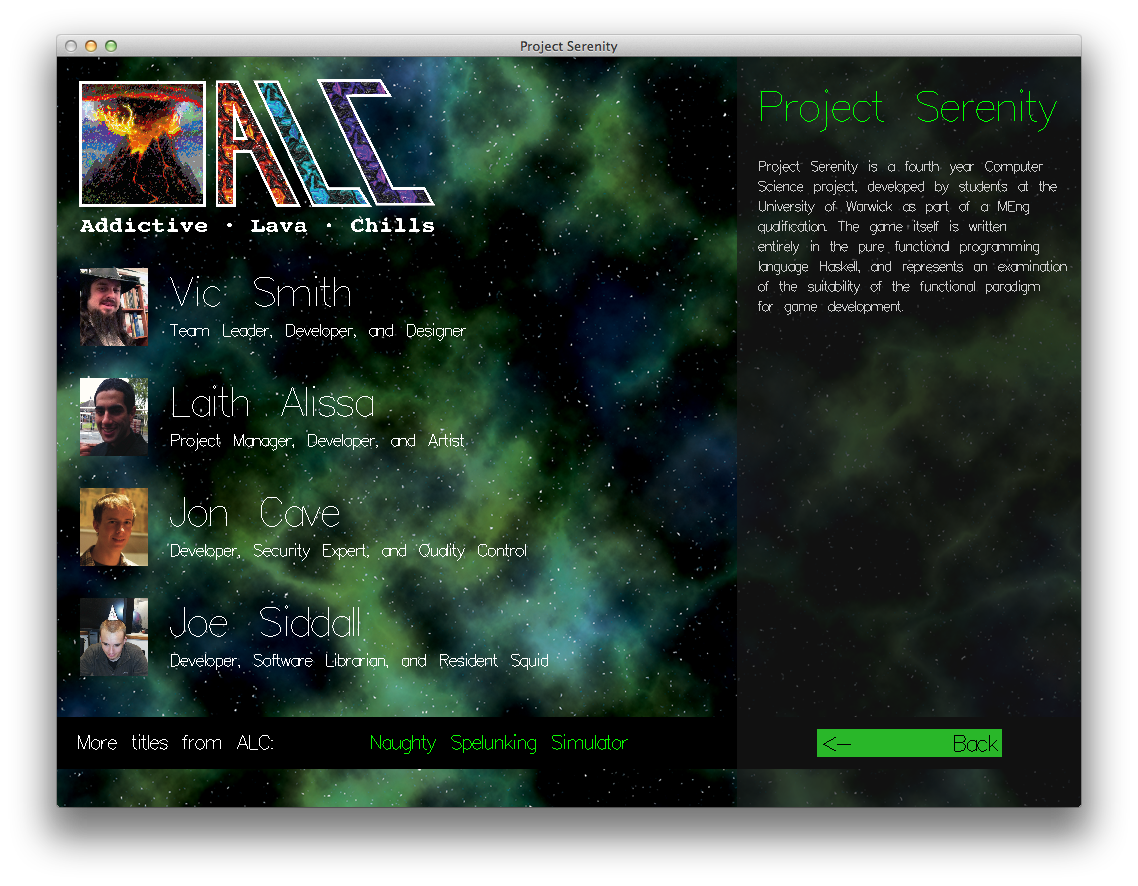
\includegraphics[width=15.5cm]{res/serenityscreens/05-credits}
	\caption[Screenshot of the credits screen]{Screenshot of the credits screen.}
	\label{fig:credits}
\end{figure*}
